%%%%%%%%%%%%%%%%%%%%%%%%%%%%%%%%%%%%%%%%%%%%%%%%%%%
%
%  New template code for TAMU Theses and Dissertations starting Spring 2021.  
%
%
%  Author: Thesis Office
%  
%  Last Updated: 1/13/2021
%
%%%%%%%%%%%%%%%%%%%%%%%%%%%%%%%%%%%%%%%%%%%%%%%%%%%

%%%%%%%%%%%%%%%%%%%%%%%%%%%%%%%%%%%%%%%%%%%%%%%%%%%%%%%%%%%%%%%%%%%%%%%
%%%                           SECTION III (This "chapter" is meant to be included in the proposal document only!)
%%%%%%%%%%%%%%%%%%%%%%%%%%%%%%%%%%%%%%%%%%%%%%%%%%%%%%%%%%%%%%%%%%%%%%


\chapter{\MakeUppercase{Proposal Methodology Plan}}
\label{cha:proposal-methodology}

Design science shall be used as the primary method of investigation in this dissertation due to its ability to derive insights from the development of new artifacts. However, design science itself is only a process that guides the investigation. To effectuate this process, the researcher has developed the following plan to build and evaluate a software system (powered by a domain-specific programming language) for potential use in the professional domain of energy market monitoring.

This plan includes the following details (illustrated by Figure \ref{fig:deliverable-plan}):

\begin{itemize}
    \item{A literature review to both introduce the research area and to establish relevance and novelty}
    \item{A Delphi-based study using a panel of experts (within market monitoring) to identify the current needs of these experts\footnote{The results of this panel shall serve as the basis for constructing a comprehensive software requirements document used during the development of this system.}, including:}
        \begin{itemize}
            \item{The current landscape of a market monitor's workflow}
            \item{Perspectives from the entire market monitoring community, including market monitors that work outside of the United States}
        \end{itemize}
    \item{A comprehensive data and system architecture plan for setting up and operating a DSL-enabled data analysis system}
    \item{Development of a prototype system to serve as a proof-of-concept for using a DSL in the context of market monitoring analysis}
    \item{Develop a \textit{traceability matrix} \cite{pm-traceability-matrix} that can serve as a method of evaluation, for this system, to ensure that the prototype serves the intended functional requirements}
    \item{A discussion of the performance of the system (as this also impacts the system's usability).}
\end{itemize}

\begin{figure}[ht]
\centering
\fbox{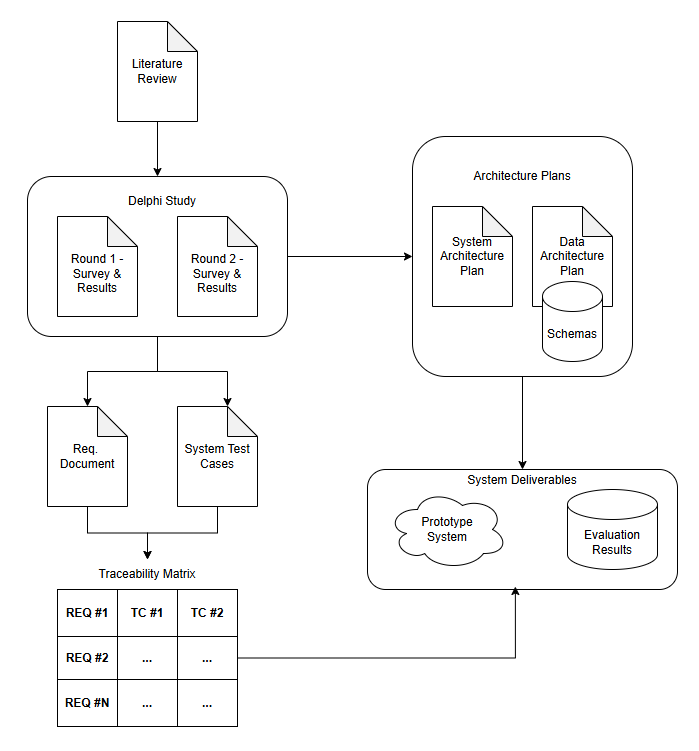
\includegraphics[scale=0.70]{graphic/deliverable_plan.png}}
\caption{Flowchart of Project Deliverables}
\label{fig:deliverable-plan}
\end{figure}

% Perforce software's definition of a Requirements Traceability Matrix --> https://www.perforce.com/resources/alm/requirements-traceability-matrix

These deliverables shall be joined together to form a software system (for which a domain-specific language is the primary user interface). To aid in drawing quantitative conclusions from this system, the researcher plans to develop a \textit{traceability matrix} from the requirements contained in the functional requirements document (FRD). This matrix will be joined to the test cases (TC) that are crafted directly from the requirements in the FRD. 

There is precedent for the use of a traceability matrix when evaluating prototypical software. Yanbin Ye, a previous student of the UA Little Rock Department of Information Science, utilized this approach in \textit{A Positive Data Control System for the Automation of Data Governance Functions}. Ye’s research identified a table of ten (10) system conditions that should be considered in the development of a data control system \cite{yanbin-ye}. Ye then evaluated this prototype to determine how closely the artifact conformed to those requirements. 

Such a scheme for system evaluation is advantageous because it helps to calculate overall system scores--- which are useful when determining if such a software application meets the needs of the intended user base. These scores are often used in information quality settings where quality is gauged on a percentage basis.

As an example, a metric that may be computed during the prototype evaluation is a \textit{conformance score} of the number of test cases that pass for a given requirement (e.g. requirement ID \textit{R1.0.0}). This example is illustrated by the following equation:

\[
\text{Conformance Score}_{\text{R1.0.0}} = 
\frac{\text{\# Test Cases Passed}}{\text{\# Total Test Cases}} 
\times 100\%
\]

Another possible evaluation score is the number of test cycles completed to ensure that all test cases pass for a specific requirement. This evaluation scheme is also helpful because the designer can justify why certain requirements may have been changed (or removed) during the design and development phases of this project.

This traceability matrix is intended to be completed in concert with the requirements document, which is ultimately dependent on the completion of the Delphi study. The requirements modeling and traceability matrix are planned to be completed in the Fall 2025 semester.
